%% generato automaticamente da tools/build_tex.py --- non modificare
\chapter{Una costruzione che si dimezza}
\label{cap:teoria2}
\quaderno{teoria2.dfw}{02 Nov 2009}{31}

Novembre 2009. Un quaderno interamente geometrico, e con una struttura ricorsiva che si scopre solo leggendolo fino in fondo. Si parte dalla bisettrice $y=x$ e da una retta perpendicolare; il loro incontro fissa un punto. Per quel punto si fa passare una parabola. Poi si abbassa la retta perpendicolare, si trova un nuovo punto — a metà distanza — e per esso si fa passare una cubica. Poi una quartica. Le ultime tre espressioni chiudono il cerchio con la formula generale per il grado $n$.

\section{Il punto di partenza}

Le prime quattro espressioni fissano la scena. La bisettrice e l'antibisettrice traslata di $k$ si incontrano in un punto che sta a distanza $k/\sqrt{2}$ dall'origine: è il vertice del quadrato di lato $k/2$ costruito sugli assi.

\begin{espr}{1}{User}{}
\[
y = x
\]
\end{espr}
La bisettrice del primo quadrante: sarà il luogo di tutti i punti di appoggio della costruzione.

\begin{espr}{2}{User}{}
\[
y = -x + k
\]
\end{espr}
La retta perpendicolare che stacca sugli assi il segmento $k$.

\begin{espr}{3}{Simp(Solve(User,[x,y]))}{}
\[
\left[\, x = \frac{k}{2} \;\land\; y = \frac{k}{2} \,\right]
\]
\end{espr}
Il loro incontro, ovviamente a metà: entrambe le coordinate valgono $k/2$.

\begin{espr}{4}{User}{}
\[
d = \frac{k}{\sqrt{2}}
\]
\end{espr}
La distanza di quel punto dall'origine, per il teorema di Pitagora sul quadrato di lato $k/2$.

\section{La parabola e il rapporto aureo}

Si cerca ora la parabola $y=ax^2$ che passa per quel punto. Il coefficiente si determina in una riga. Poi si abbassa la retta e si chiede dove incontri la parabola: la risposta contiene una sorpresa.

\begin{espr}{5}{User}{}
\[
y = a\, x^{2}
\]
\end{espr}
Si introduce la famiglia delle parabole per l'origine.

\begin{espr}{6}{User}{}
\[
\frac{k}{2} = a\, \left(\frac{k}{2}\right)^{2}
\]
\end{espr}
Si impone il passaggio per il punto trovato.

\begin{espr}{7}{User}{}
\[
a = \frac{2}{k}
\]
\end{espr}
Il coefficiente che ne risulta.

\begin{espr}{8}{User}{}
\[
y = \frac{2}{k}\, x^{2}
\]
\end{espr}
La parabola determinata. Con $k=1$ diventa $y=2x^2$.

\begin{espr}{9}{User}{}
\[
y = -x + \frac{k}{2}
\]
\end{espr}
La retta si abbassa: il termine noto passa da $k$ a $k/2$.

\begin{espr}{10}{User}{}
\[
x = k\, \left(\frac{\sqrt{5}}{4} - \frac{1}{4}\right) \;\land\; y = k\, \left(\frac{3}{4} - \frac{\sqrt{5}}{4}\right)
\]
\end{espr}
L'intersezione della parabola con la retta abbassata, dove compare $\sqrt5$.

\begin{espr}{11}{User}{}
\[
\left[\, x = \frac{k}{4} \;\land\; y = \frac{k}{4} \,\right]
\]
\end{espr}
L'intersezione della retta abbassata con la bisettrice: il nuovo punto di appoggio, a coordinate $k/4$. È questo, non il precedente, a generare il passo successivo.


L'ascissa dell'intersezione, $\#10$, vale $k(\sqrt5-1)/4$. Il fattore $(\sqrt5-1)/2$ è l'inverso del rapporto aureo, $1/\varphi\approx 0{,}618$: la parabola taglia la retta abbassata in un punto che divide il segmento in proporzione aurea. Non è una coincidenza costruita apposta — emerge dall'equazione $2x^2+kx-k^2/2=0$, il cui discriminante è $5k^2$. Il quaderno non commenta il fatto e passa oltre.

\section{La cubica}

Il punto $\#11$, che sta a metà strada rispetto al precedente, diventa il nuovo appoggio: per esso passa una cubica. La struttura del passaggio è identica a quella della parabola, e questo è il segnale che si tratta di una ricorsione.

\begin{espr}{12}{User}{}
\[
y = a\, x^{3}
\]
\end{espr}
La famiglia delle cubiche.

\begin{espr}{13}{User}{}
\[
\frac{k}{4} = a\, \left(\frac{k}{4}\right)^{3}
\]
\end{espr}
Il passaggio imposto per il punto a coordinate $k/4$.

\begin{espr}{14}{User}{}
\[
a = \frac{16}{k^{2}}
\]
\end{espr}
Il coefficiente: $16/k^2$, cioè $2^4$ diviso $k^2$.

\begin{espr}{15}{User}{}
\[
y = \frac{16}{k^{2}}\, x^{3}
\]
\end{espr}
La cubica determinata.

\begin{espr}{16}{User}{}
\[
y = -x + \frac{k}{4}
\]
\end{espr}
La retta si abbassa ancora, a $k/4$.

\begin{espr}{17}{Simp(User)}{}
\[
x = k\, \left(\left(\frac{\sqrt{93}}{1152} + \frac{1}{128}\right)^{\frac{1}{3}} - \left(\frac{\sqrt{93}}{1152} - \frac{1}{128}\right)^{\frac{1}{3}}\right) \;\land\; y = k\, \left(\left(\frac{\sqrt{93}}{1152} - \frac{1}{128}\right)^{\frac{1}{3}} - \left(\frac{\sqrt{93}}{1152} + \frac{1}{128}\right)^{\frac{1}{3}} + \frac{1}{4}\right)
\]
\end{espr}
L'intersezione, in forma di Cardano. I due radicandi differiscono solo per il segno del termine $1/128$, come è tipico della formula risolutiva del terzo grado.


L'espressione $\#17$ è la soluzione di Cardano dell'equazione $16x^3+x-k/4=0$: due radici cubiche di binomi che contengono $\sqrt{93}$. Il contrasto con il caso quadratico è istruttivo — stessa costruzione, un grado in più, e la soluzione passa da $\sqrt5$ a una forma irriducibile in radicali annidati.

\section{I casi particolari con $k=1$}

Una breve pausa di verifica: le stesse curve e le stesse rette scritte con $k=1$, per poterle disegnare. Sono le espressioni che il quaderno mandava alla finestra grafica.

\begin{espr}{18}{User}{}
\[
y = 16\, x^{3}
\]
\end{espr}
La cubica con $k=1$.

\begin{espr}{19}{User}{}
\[
y = -x + \frac{1}{4}
\]
\end{espr}
La retta corrispondente, pronta per il grafico.

\begin{espr}{20}{User}{}
\[
y = 2\, x^{2}
\]
\end{espr}
La parabola con $k=1$.

\begin{espr}{21}{User}{}
\[
y = -x + \frac{1}{2}
\]
\end{espr}
La sua retta.

\begin{espr}{22}{User}{}
\[
y = x
\]
\end{espr}
La bisettrice, che nella costruzione è la curva di grado uno.

\begin{espr}{23}{User}{}
\[
y = -x + 1
\]
\end{espr}
E la retta di partenza, con $k=1$: il caso $n=1$ della famiglia generale.

\section{La quartica e la legge generale}

L'ultimo giro della ricorsione, e poi la formula che li racchiude tutti.

\begin{espr}{24}{User}{}
\[
y = a\, x^{4}
\]
\end{espr}
Si passa al quarto grado.

\begin{espr}{25}{User}{}
\[
\frac{k}{8} = a\, \left(\frac{k}{8}\right)^{4}
\]
\end{espr}
Il punto di appoggio è ora a coordinate $k/8$: ogni passo dimezza.

\begin{espr}{26}{User}{}
\[
a = \frac{512}{k^{3}}
\]
\end{espr}
Il coefficiente $512=2^9$.

\begin{espr}{27}{User}{}
\[
y = \frac{512}{k^{3}}\, x^{4}
\]
\end{espr}
La quartica determinata.

\begin{espr}{28}{User}{}
\[
y = -x + \frac{1}{8}
\]
\end{espr}
La retta corrispondente.

\begin{espr}{29}{User}{}
\[
a = \frac{2^{\left(n - 1\right)^{2}}}{k^{n - 1}}
\]
\end{espr}
La legge generale del coefficiente. L'esponente $(n-1)^2$ dà $2^0,\ 2^1,\ 2^4,\ 2^9,\ 2^{16}$ per $n=1,2,3,4,5$.

\begin{espr}{30}{User}{}
\[
y = \frac{2^{\left(n - 1\right)^{2}}}{k^{n - 1}}\, x^{n}
\]
\end{espr}
La famiglia completa di curve.

\begin{espr}{31}{User}{}
\[
y = -x + 2^{1 - n}
\]
\end{espr}
E la famiglia di rette che le accompagna. Il termine noto $2^{1-n}$ genera il punto di appoggio del grado successivo, non di quello corrente: è questo sfasamento a rendere la costruzione una ricorsione anziché una semplice sostituzione.

\begin{figure}[htbp]
  \centering
  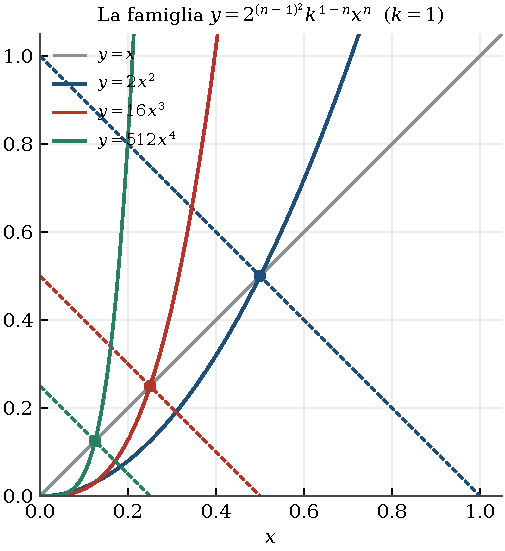
\includegraphics[width=0.66\linewidth]{../figures/teoria2.pdf}
  \caption{La costruzione con $k=1$. Ogni curva incontra la bisettrice in un punto che dista dall'origine la metà del precedente; la retta tratteggiata dello stesso colore è quella che ha generato il punto di appoggio.}
  \label{fig:teoria2}
\end{figure}

La formula $\#29$ è il punto di arrivo. Il coefficiente $a=2^{(n-1)^2}k^{1-n}$ è esattamente quello che serve perché la curva $y=ax^n$ passi per il punto $\left(k/2^{\,n-1},\ k/2^{\,n-1}\right)$: imponendo $p=ap^n$ con $p=k/2^{\,n-1}$ si ricava $a=p^{1-n}$, e sviluppando la potenza compare l'esponente quadratico $(n-1)^2$. La crescita è impressionante: $2$, $16$, $512$, $65\,536$, e al passo successivo già oltre trentatré milioni. Ogni grado in più costringe la curva a stare più aderente all'asse per poi risalire fino alla bisettrice in un punto due volte più vicino all'origine.

\section*{In sintesi}
\addcontentsline{toc}{section}{In sintesi}

Trentuno espressioni per una sola idea, sviluppata con pazienza: una successione di curve di grado crescente ancorate a punti che si avvicinano geometricamente all'origine. Il risultato finale, $a=2^{(n-1)^2}k^{1-n}$, è compatto e si verifica in una riga; ma il modo in cui il quaderno ci arriva — un caso, poi un altro, poi un terzo, e solo allora la formula — è il modo in cui le regolarità si trovano davvero.

